\section{Durchführung}
\label{sec:Durchführung}
Zur Vermessung der Körper werden diese auf einer 
Drillachse (siehe Abbildung \ref{fig:a}) befestigt.
Doch um die Trägheitsmomente der Körper zu bestimmen
muss zunächst die Drillachse an sich untersucht werden.

\begin{figure}[H]
    \centering
    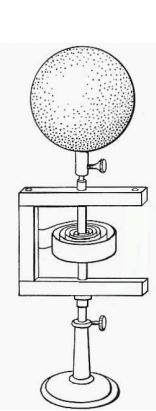
\includegraphics[width=3cm]{content/Drill.png}
    \caption{Drillachse mit Vollkugel \cite{sample}}
    \label{fig:a}
\end{figure}


\subsection{Vermessung der Drillachse}
\begin{figure}[H]
    \centering
    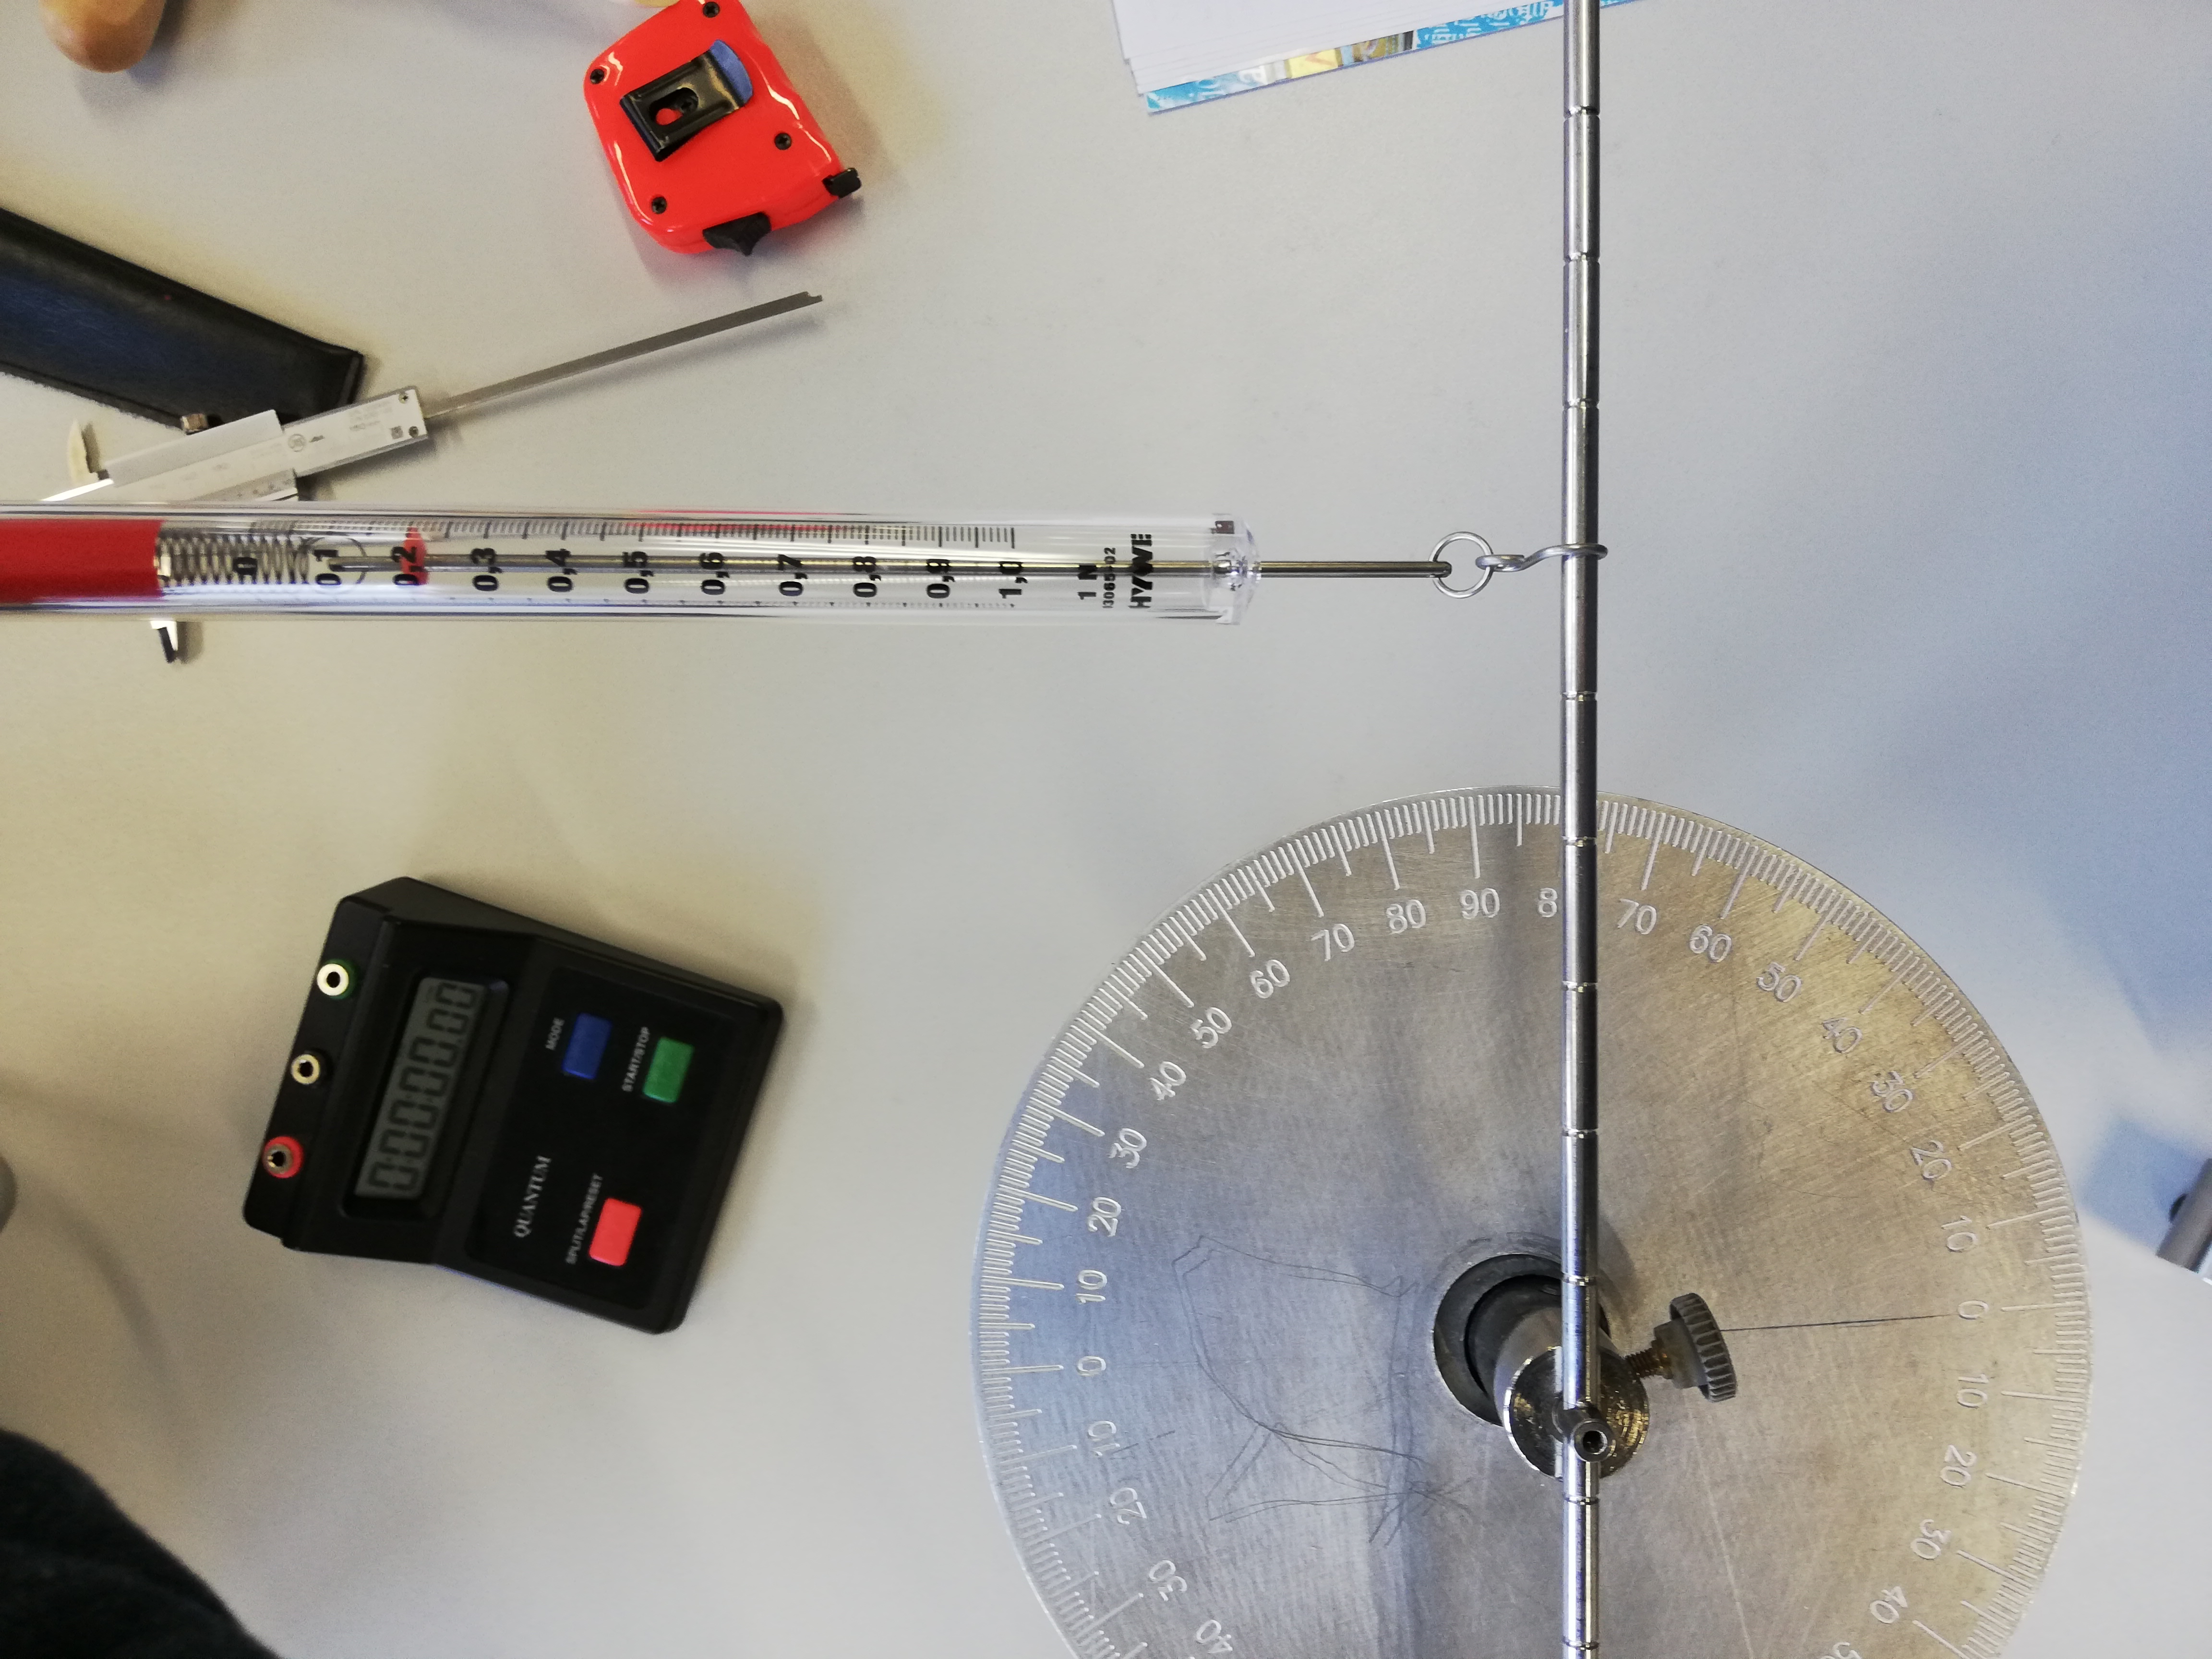
\includegraphics[width=8cm]{content/1.jpg}
    \caption{Bestimmung der Winkelrichtgröße $D$ einer Drillachse}
    \label{fig:b}
\end{figure}

\noindent Mit dem Aufbau in Abbildung \ref{fig:b}
kann die Winkelrichtgröße $D$ bestimmt werden. Dazu wird
mit Hilfe eines Kraftmessers  in einem Abstand
von $r=12\,\si{\centi\meter}$ die Rückstellende Kraft 
der Feder bei 10 unterschiedlichen Auslenkungen gemessen.

\begin{figure}[H]
    \centering
    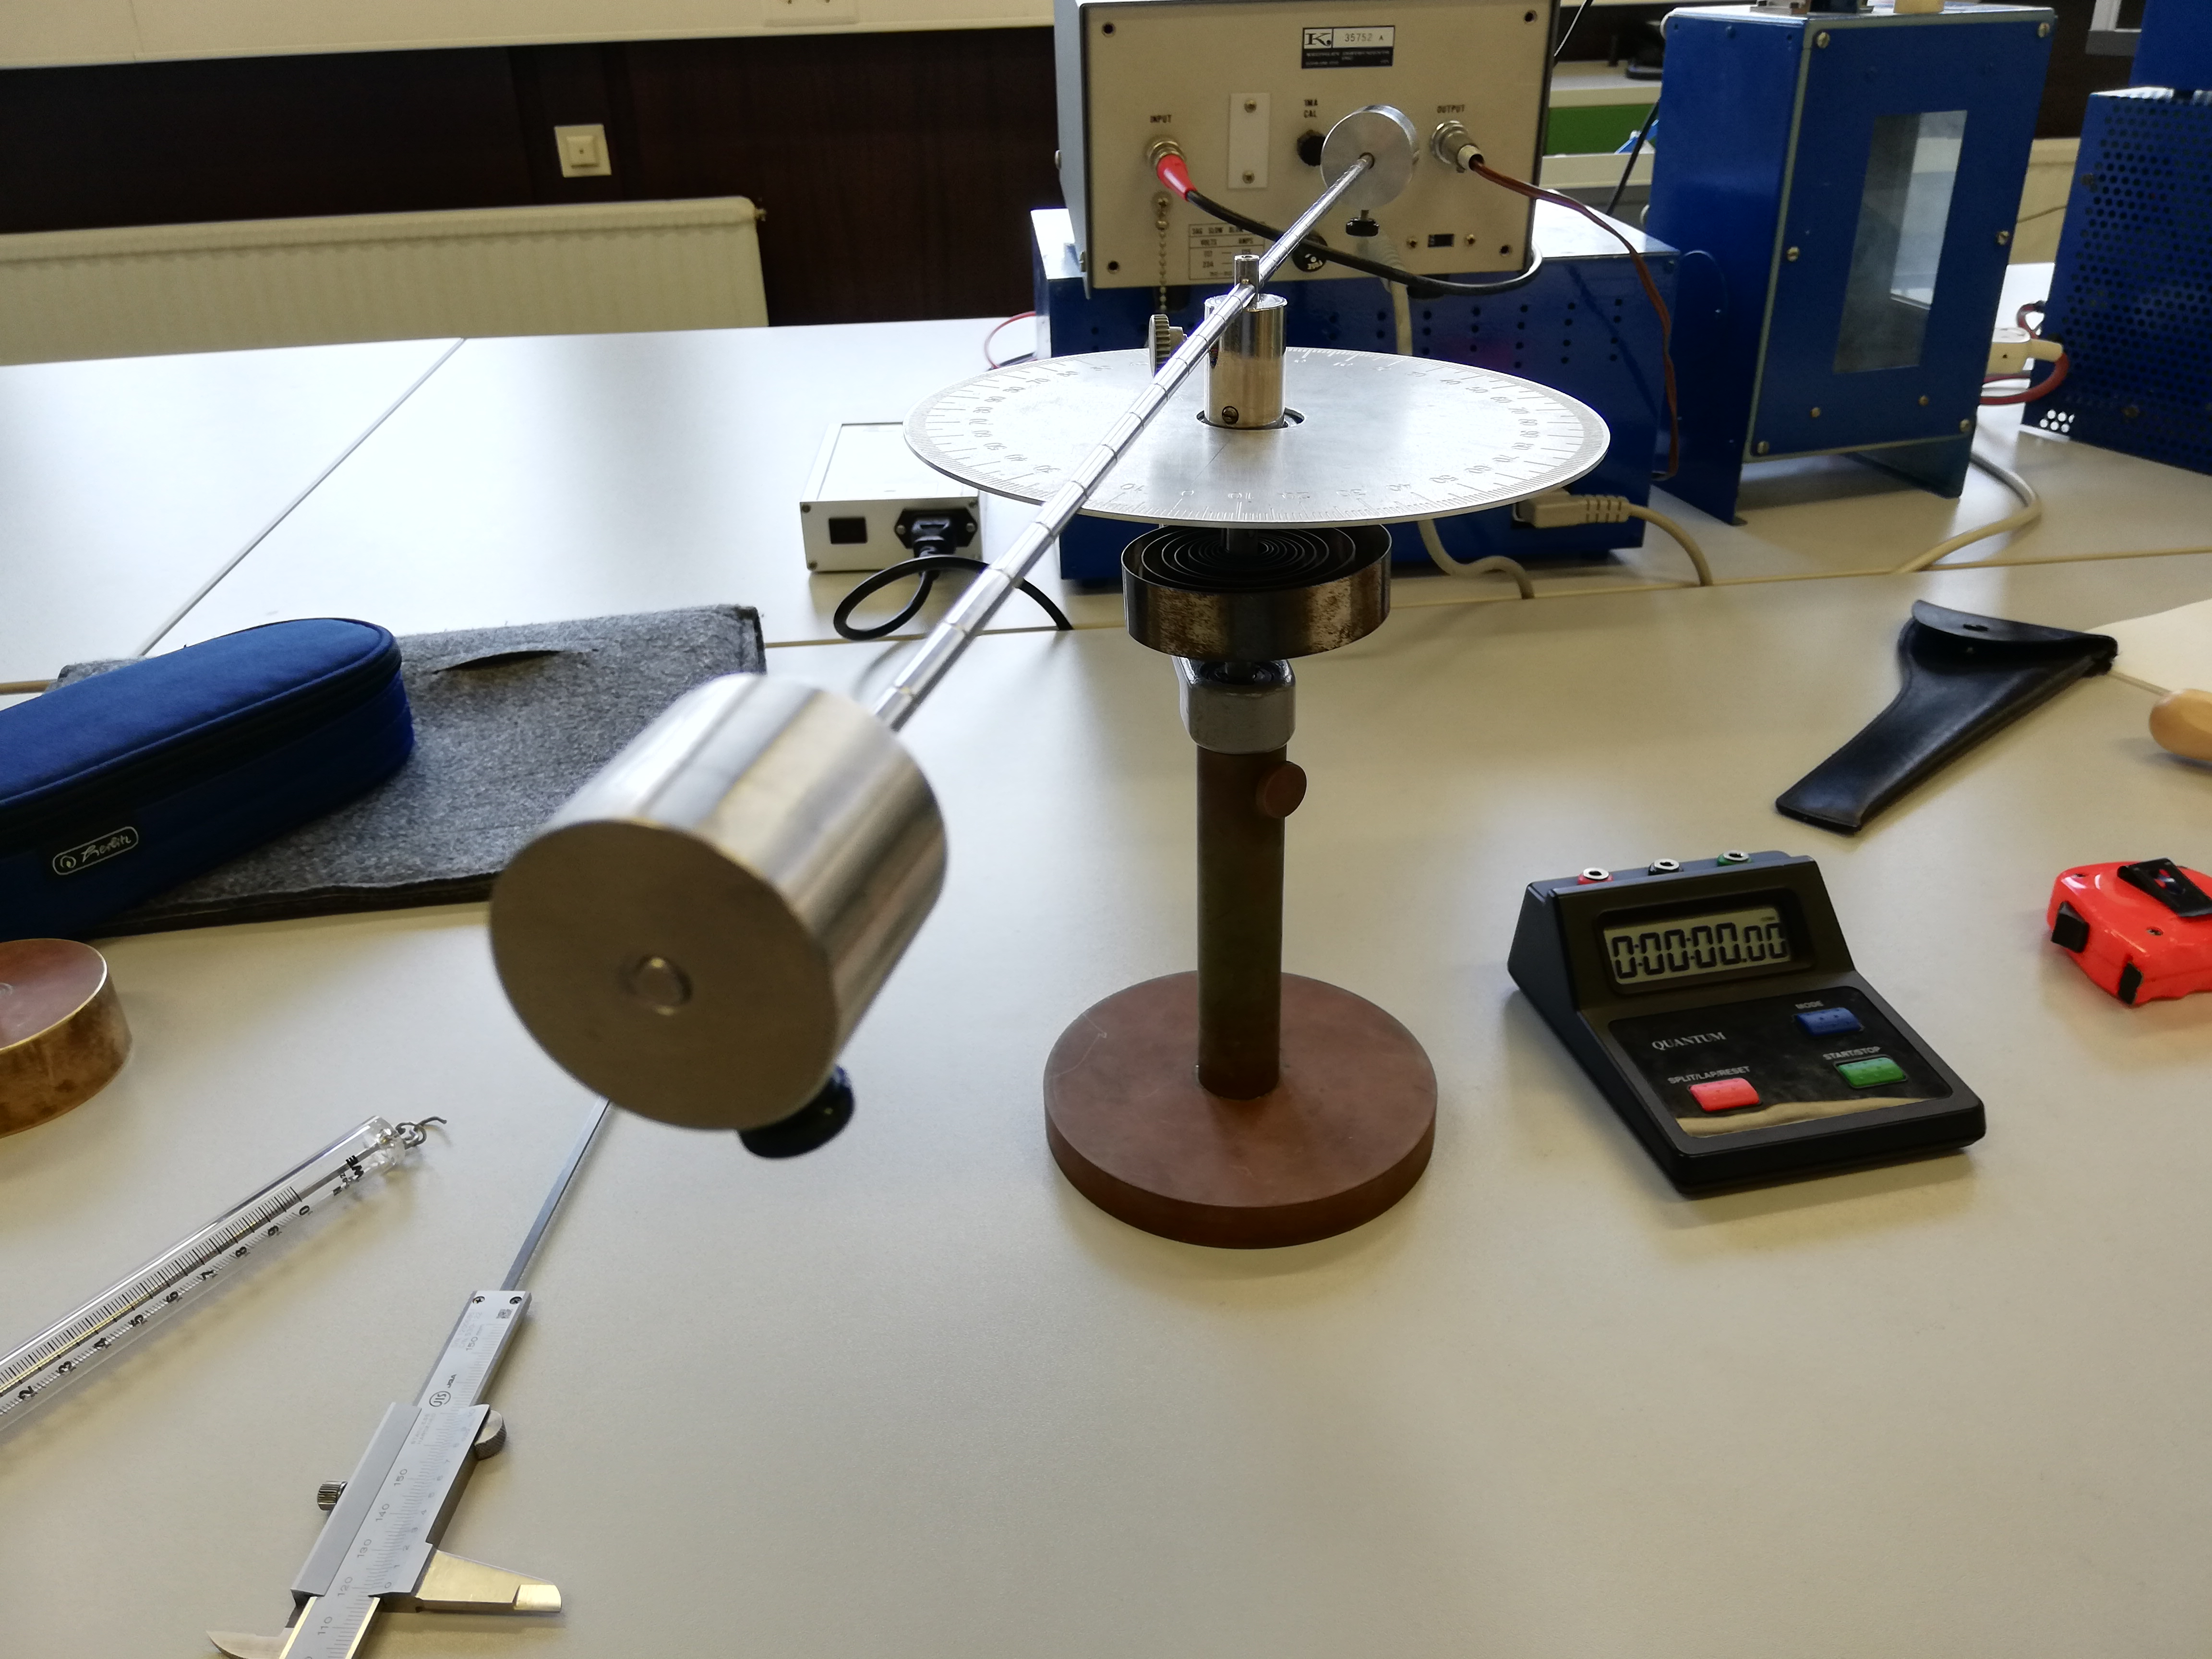
\includegraphics[width=8cm]{content/2.jpg}
    \caption{Bestimmung des Eigenträgheitsmoment $I_D$ einer Drillachse}
    \label{fig:b}
\end{figure}

\noindent Zur Bestimmung des Eigenträgheitsmoment der
Drillachse werden zwei Zylinder mit $m=222,9\,\si{\gram}$ und $R=1,995\,\si{\centi\meter}$ an einer nahezu
masselosen Stange auf der Drillachse befestigt. Nun
kann die Schwingungsdauer $T$ bei einer immer gleichen
Auslenkung von $\phi=15\,\si{\degree}$ bei 10 unterschiedlichen Abständen der
Zylinder voneinander gemessen werden.



\subsection{Bestimmung des Trägheitsmoments zweier Körper}
\begin{figure}[H]
    \centering
    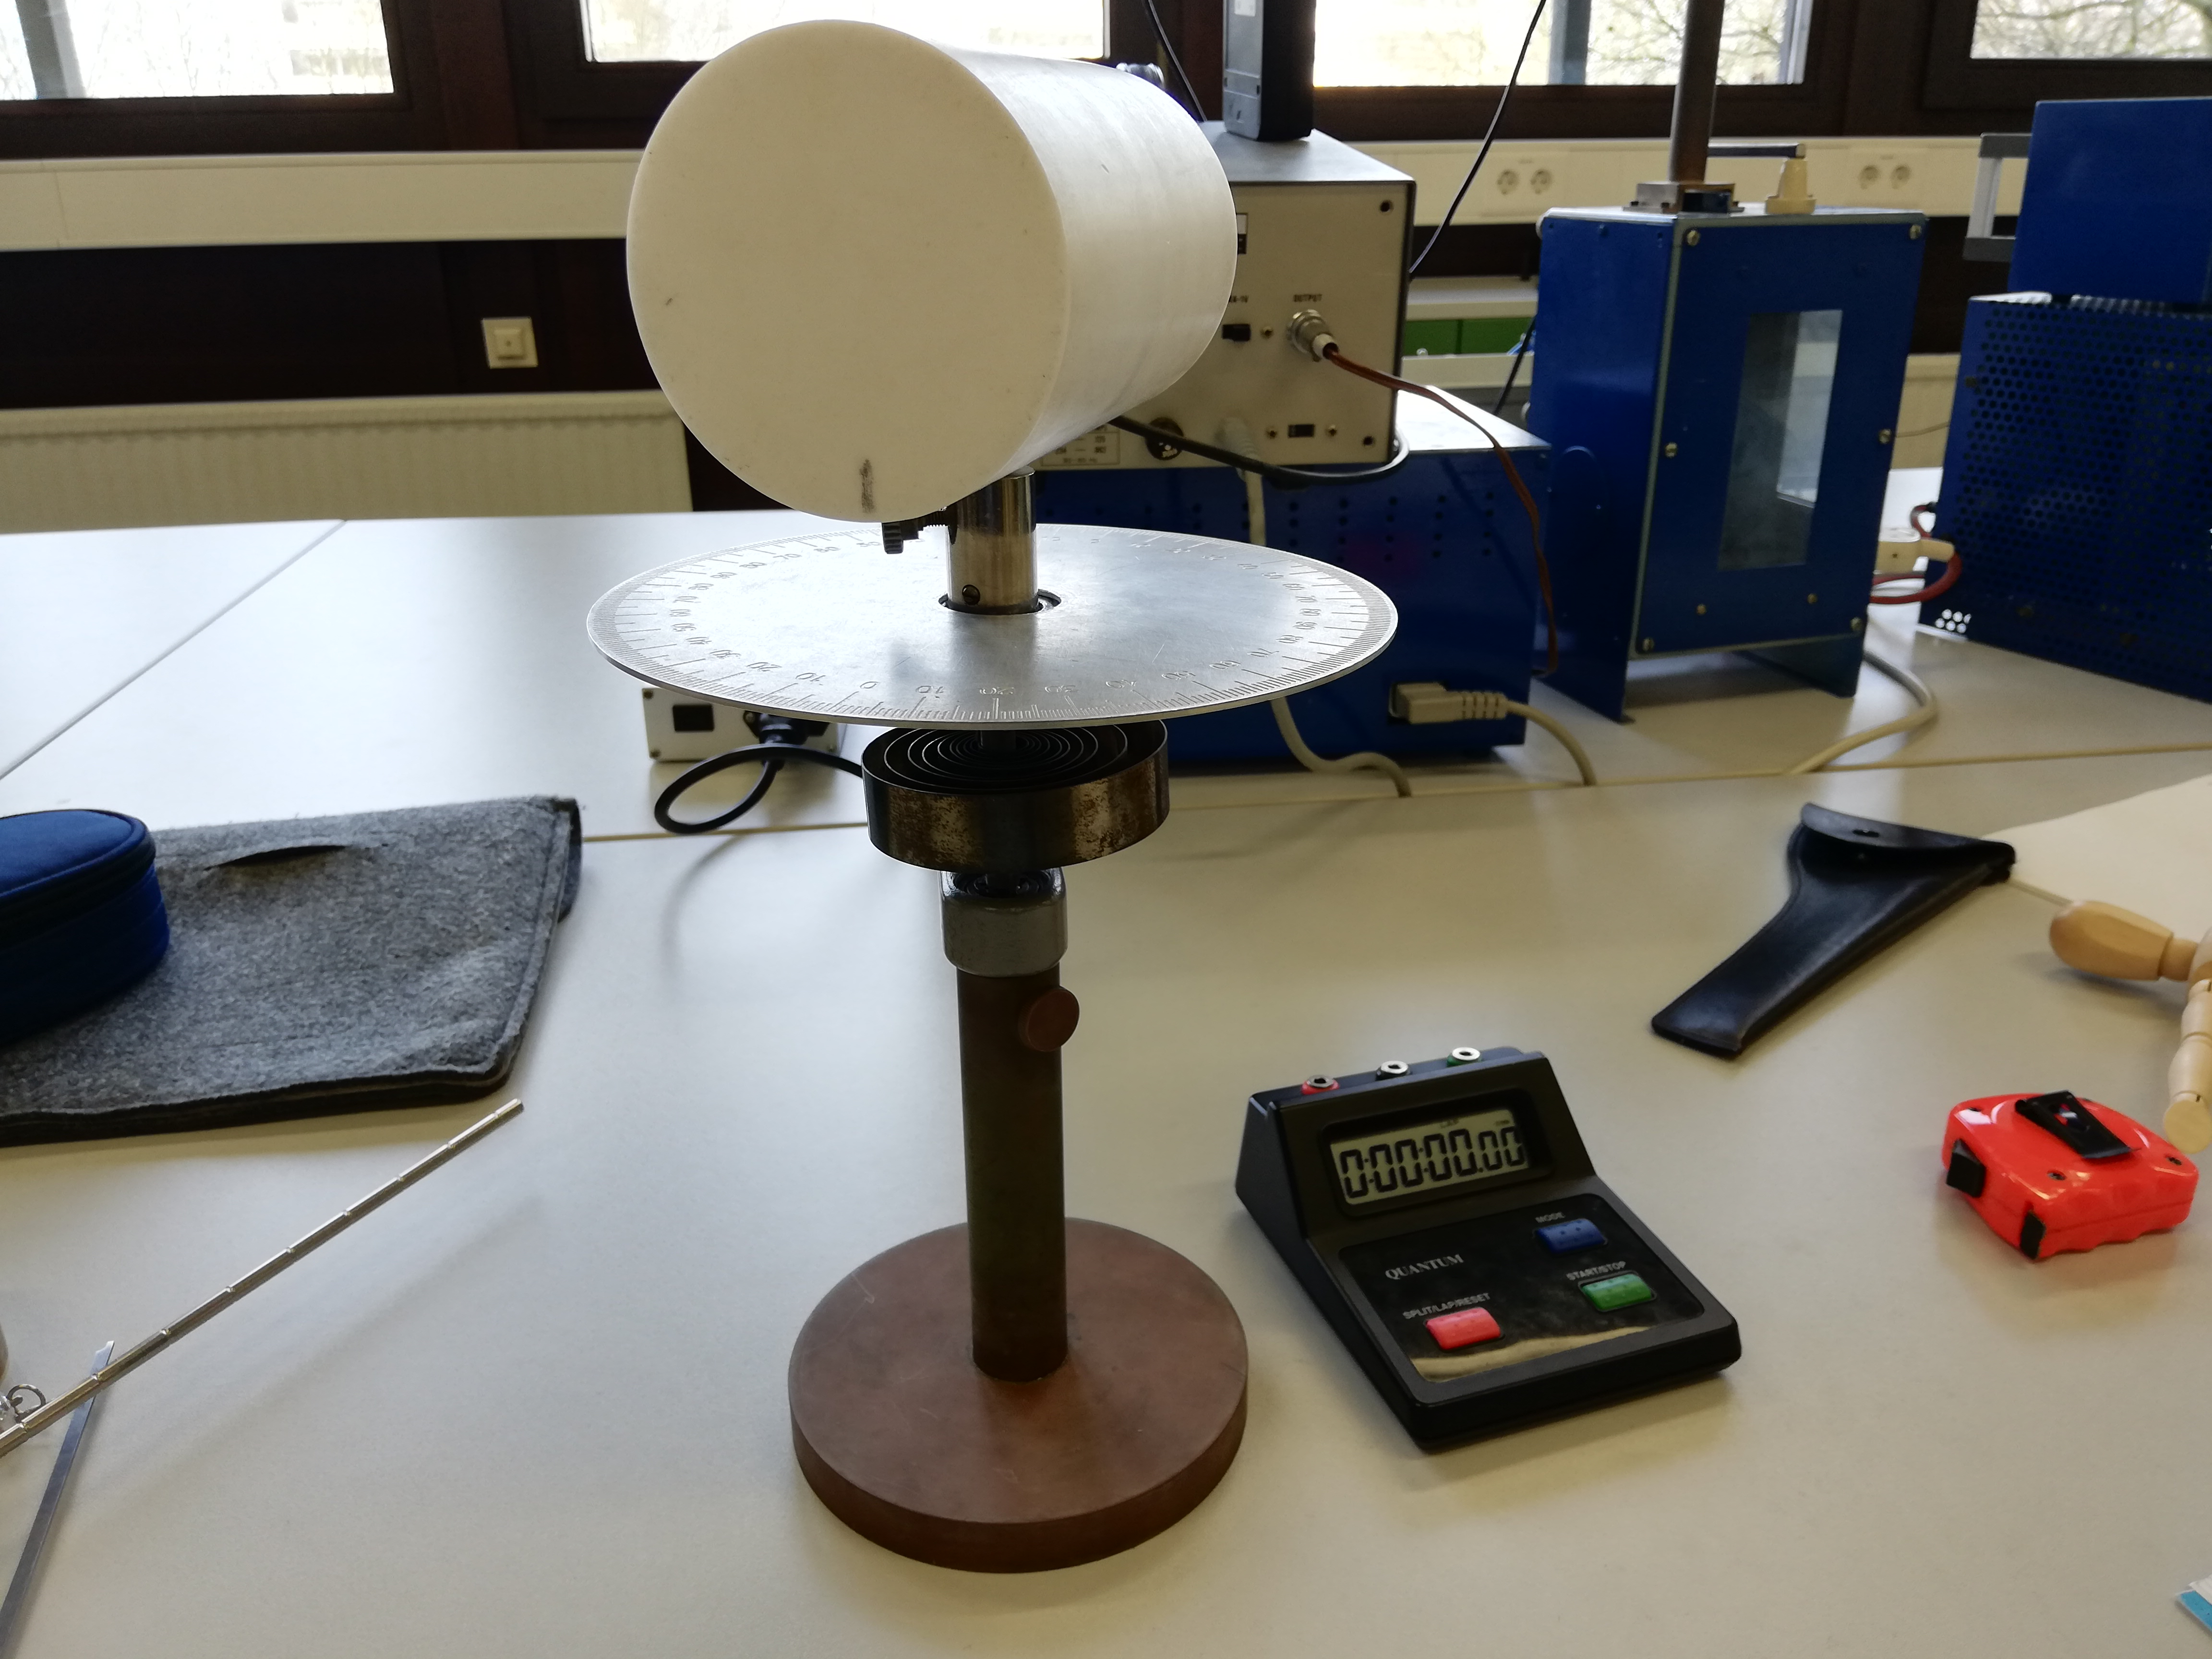
\includegraphics[width=8cm]{content/3.jpg}
    \caption{Bestimmung des Trägheitsmoments $I$ eines Körpers mit Hilfe einer Drillachse}
    \label{fig:b}
\end{figure}
Die beiden Körper sind Zylinder, wobei sich der erste 
($R=3,75\,\si{\centi\meter}$, $m=1119,3\,\si{\gram}$)
um seine Symmetrieachse und der zweite 
($R=4,00\,\si{\centi\meter}$, $h=13,94\,\si{\centi\meter}$, $m=1525,5\,\si{\gram}$)
senkrecht zu seiner Symmetrieachse dreht. Um
das Trägheitsmoment bestimmen zu können wird jeweils
fünf mal die Schwingungsdauer bei einer Auslenkung
von $\phi=15\,\si{\degree}$ gemessen.


\subsection{Bestimmung des Trägheitsmoments einer Holzpuppe in verschiedenen Positionen}

\begin{figure}[H]
    \centering
    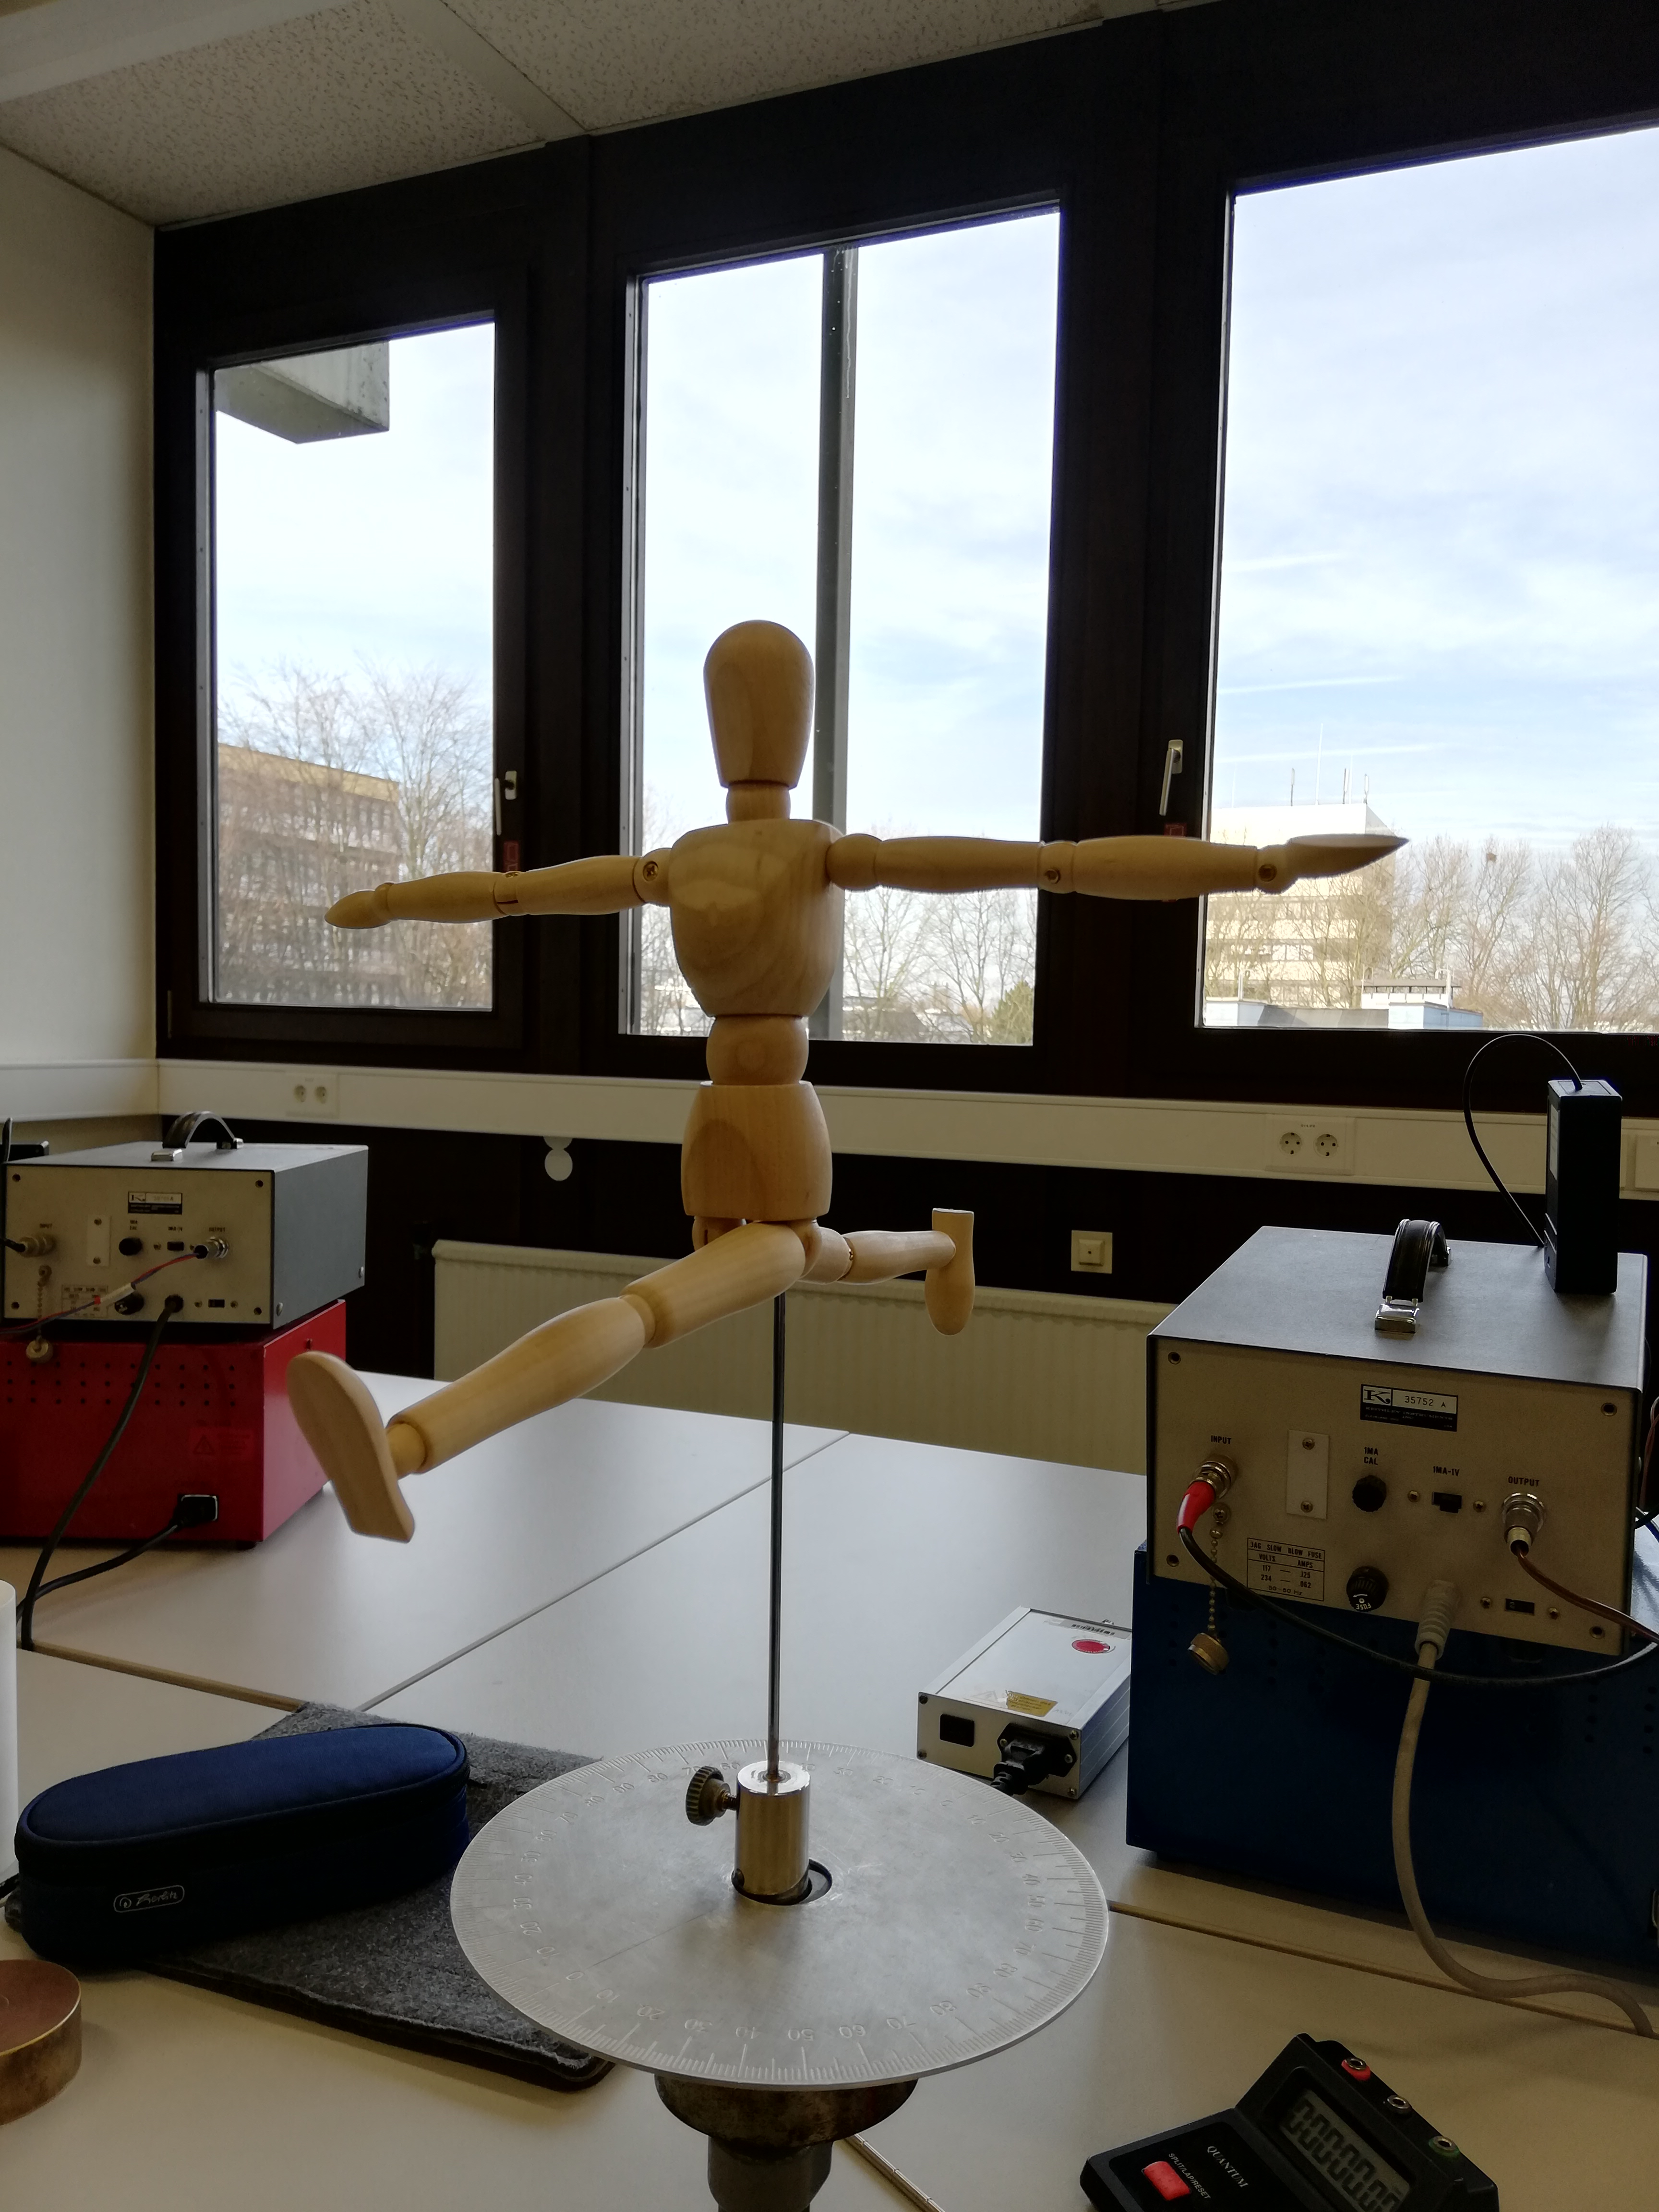
\includegraphics[width=8cm]{content/4.jpg}
    \caption{Position 1 der Holzpuppe}
    \label{fig:c}
\end{figure}

\begin{figure}[H]
    \centering
    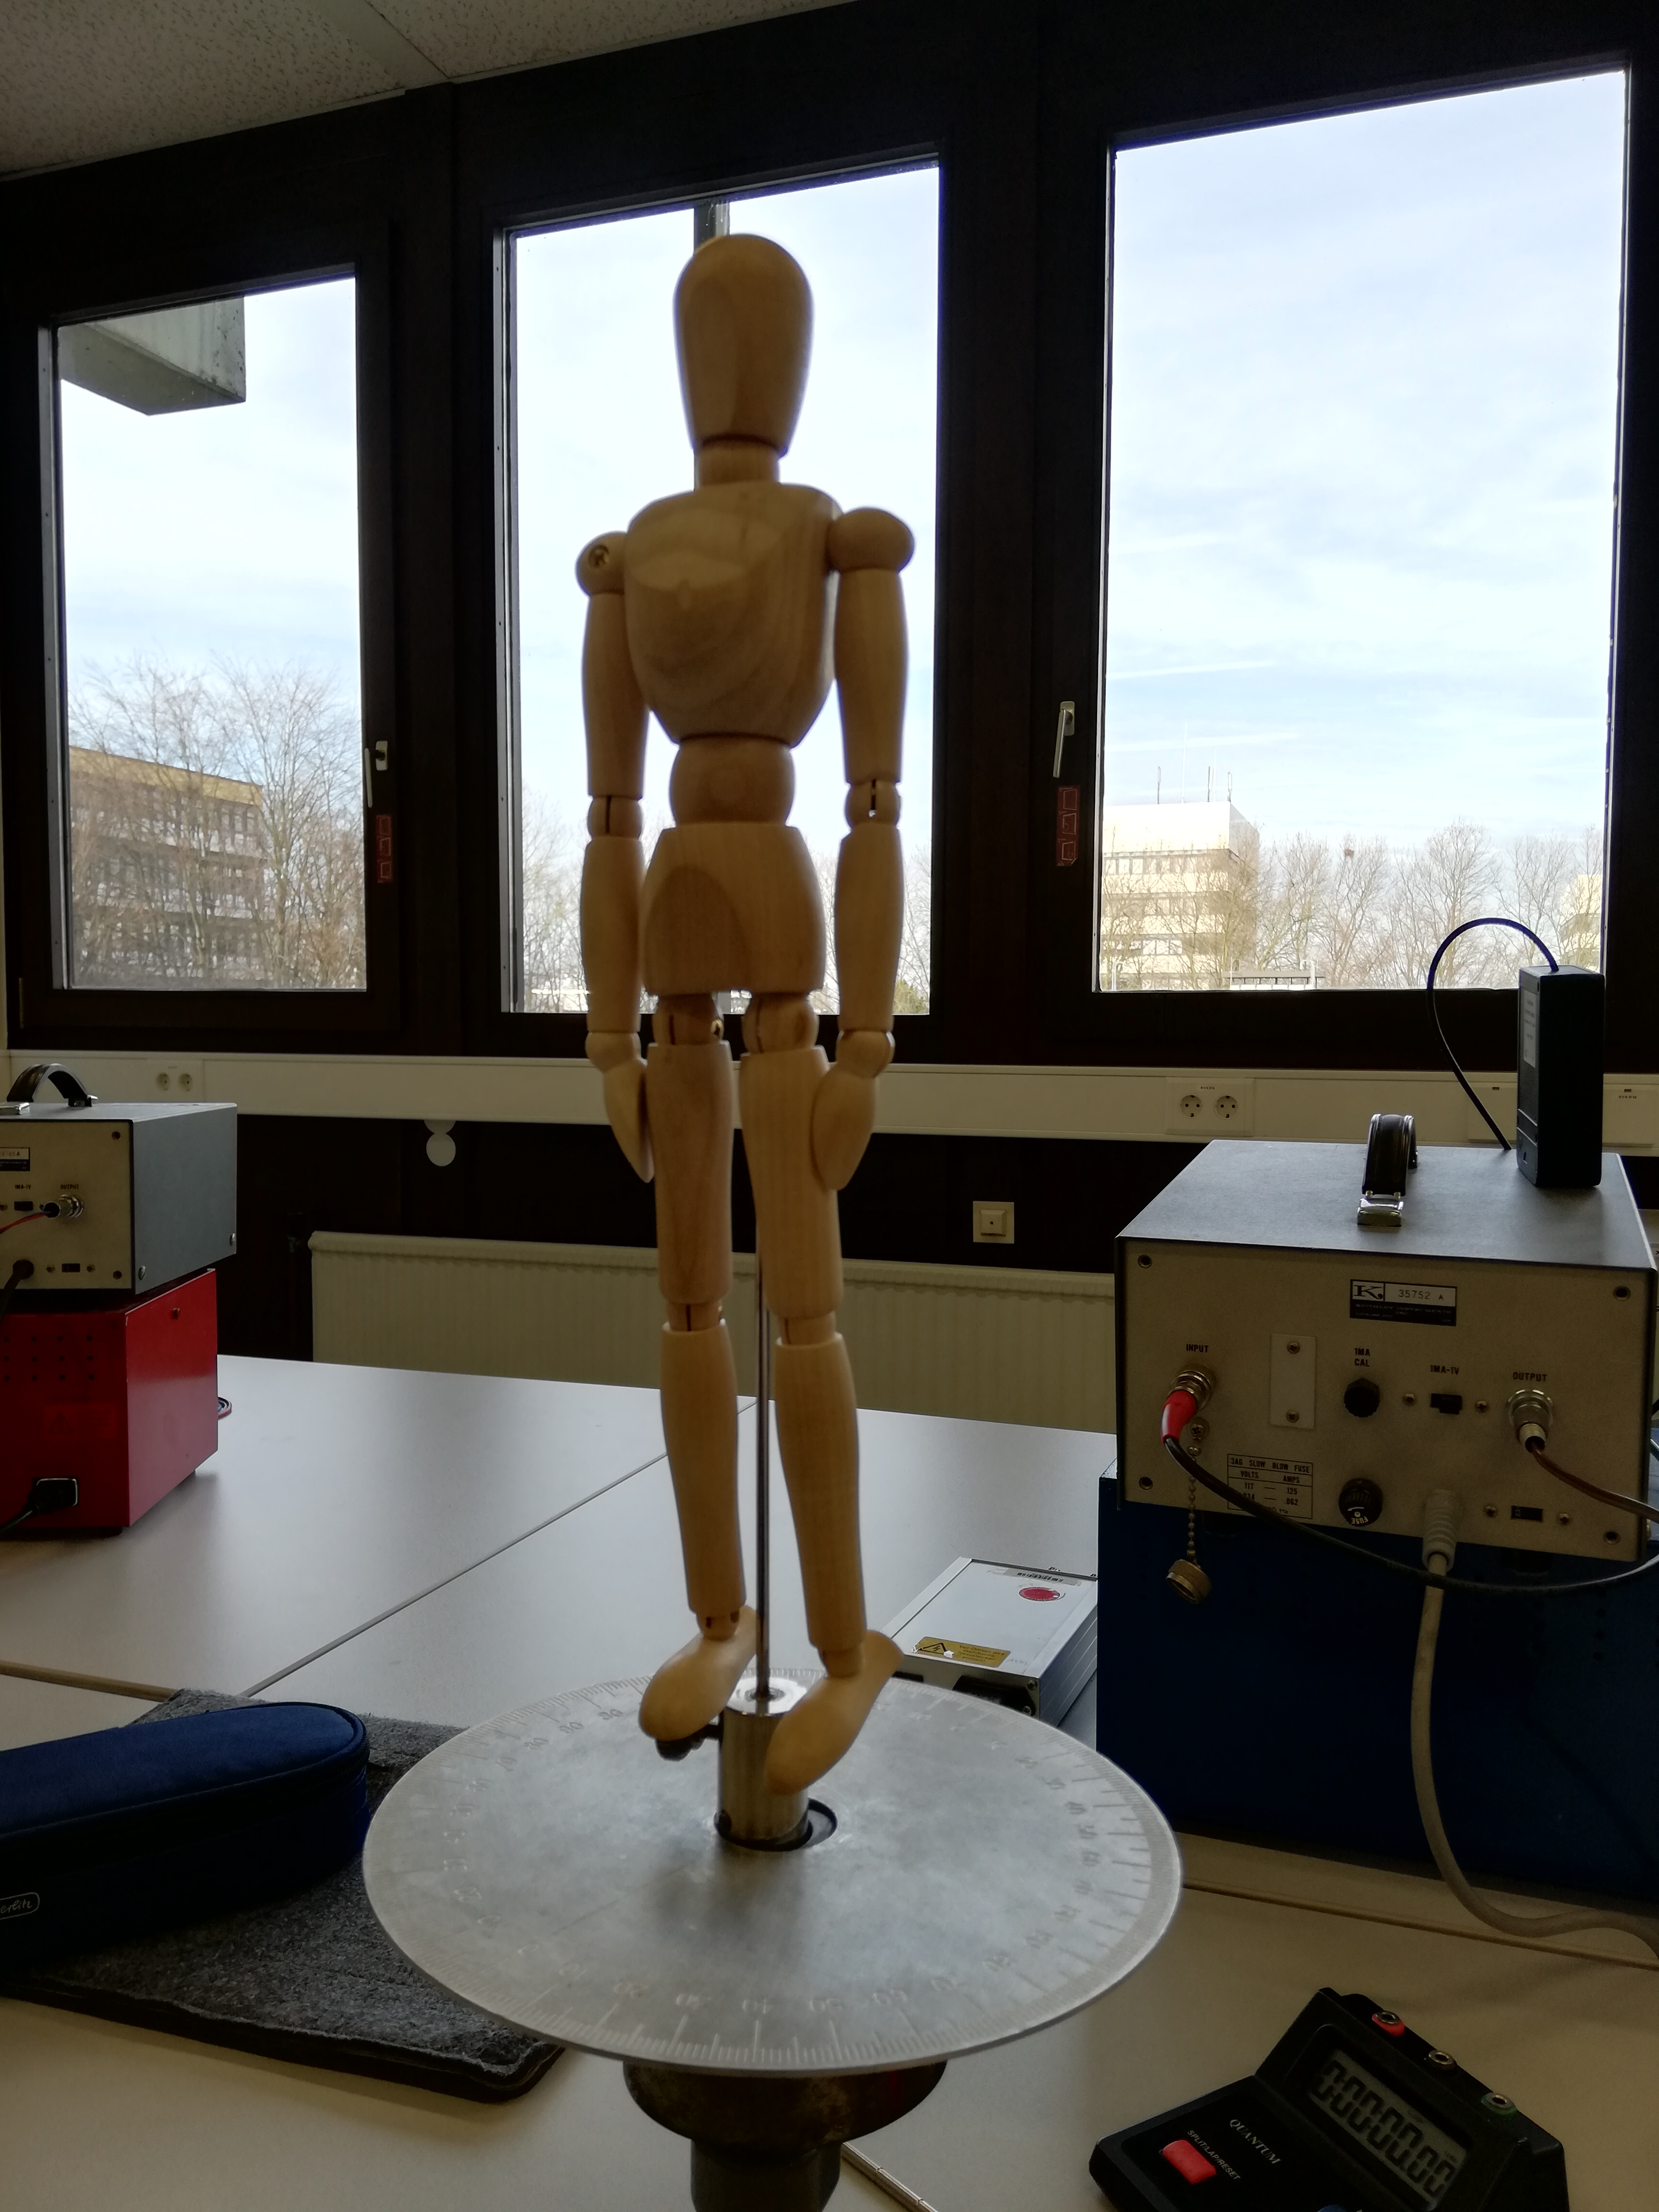
\includegraphics[width=8cm]{content/5.jpg}
    \caption{Position 2 der Holzpuppe}
    \label{fig:d}
\end{figure}


Auch bei der Holzpuppe werden pro Position fünf
Messungen vorgenommen. Dieses mal jedoch bei einer
Auslenkung von $\phi=20\,\si{\degree}$, da die
Messung der Schwingungsdauer mit einer Stoppuhr
erfolgt und bei einer zu geringen Auslenkung nicht
genau genug messbar wäre.

Der Kopf der Puppe wird durch eine Vollkugel mit 
Radius $R=1,62\,\si{\centi\meter}$ angenähert.
Die Arme werden durch Zylinder mit Radius $R=0,65\,\si{\centi\meter}$
und Länge $h=12,61\,\si{\centi\meter}$, sowie die
Beine als Zylinder mit Radius $R=0,71\,\si{\centi\meter}$
und Länge $h=14,84\,\si{\centi\meter}$ beschrieben.
Auch der Oberkörper wird durch einen Zylinder mit 
Radius $R=1,85\,\si{\centi\meter}$
und Länge $h=9,96\,\si{\centi\meter}$
